\chapter{Method}


Several hypotheses were tested in this work.
Section \ref{data_pp} gives an overview of how input data was pre-processed.
Section \ref{architecture} describes the technical set up required for running all these experiments and deploying the model to production before delving into the specific experiments and their evaluation in section \ref{exp}.

\hfill \break \noindent
The experiments were conducted in four distinct stages:

 \begin{itemize}
   \item
    Training a baseline model on the rule-based labels to get a sense of the difficulty of this problem.
    Exploring the predictions subjectively.
   \item Building a visual similarity feature and evaluating its results subjectively.
   % Since there is no fundamental difference in the way this model was  trained and evaluated compared to the other classifiers, this is described in section \ref{exp_models} with the others. After this step, employees of the client company labeled products that would become the ground truth dataset. The visual comparison feature was also subjectively evaluated at this stage.
   \item
    Training the independent classifiers to determine best performers (\ref{exp_models}).
    Due to the good perforance of individual models, ensembling was not attempted due to the engineering overhead it would incur.
    Experimenting with different multi-objective training approaches.
   \item Training [TODO] iterations of active learning on the strong predictor (\ref{exp_al}).
 \end{itemize}


 \section{Data Preprocessing}
 \label{data_pp}

There were around a dozen product features that affiliate networks provided.
Most of these features were either categorical or textual,  with just a single numerical feature.
Initially, the data was analysed using Dataprep, a Google Cloud Platform (GCP)  product for data wrangling, which at the time of use was in beta stage.
Dataprep  was used to process a sample of ~800 000 products;  it produced histograms of the values present in each feature column (see appendix \ref{dataprep}).

The histograms revealed that a lot of the input features were mostly empty, but also that many of the inputs that would naturally be considered categorical  had much more unique value in them then one might expect.
For example, each affiliate gives us the textual representation what they consider to be the category of the product,  but  rather than containing a small number of unique tokens, these contained all the full category paths along with the category delimiters, which  varied retailer by retailer (e.g.  it was common to see both ``Shoes > Sneakers'' and ``Shoes // Sneakers'').
Representing these as categorical variables would have blown up the input space, which would have  resulted in more parameters, each parameter having fewer examples to learn from.
Therefore, many such ``categorical''  were actually represented as text, which were tokenised and cleaned appropriately, allowing for better generalisation and smaller models.

There was a single numerical field: price.
This could have been min-max normalised to the range 0 ... 1, however there  was a small number of very high values that would have squash nearly all the other  prices.
Rather than  carefully considering  how to mitigate this,  the input dimension was dropped, because it is not likely to have much predictive value for product classification.
It would be trivial to bring this feature back for a training objective for which it would be much more useful.

A trickier question was how many distinct tokens or categorical values to keep per input column.
Keeping all of them would not have been sensible: there were still large numbers of tokens that appeared only once, often because there were some unwanted formatting characters, misspellings, or incorrect punctuation that caused a token to be considered a separate entity.
There was a single configuration file that dictated which models used which features as input, whether those inputs were represented as textual, categorical, or dense values;  it also determined  the maximum number of unique values/tokens,  and the dimensionality of the embedding.
This configuration file was read by Dataflow during pre-processing  and by TensorFlow during  inference and training, which made experimentation with  different types of models and input representations considerably easier.

Below is a list of input features with information about how they were represented; it also lists the dimensionality of embeddings  for the models which  encoded categorical variables as embedding.

\begin{itemize}[noitemsep]
  \item title - text - max 8000 unique tokens
  \item brand - categorical - max 5000 unique values - 10 embedding dimensions
  \item category - categorical - max 950 unique values - 6 embedding dimensions
  \item rawCategory - text - max 1000 unique tokens
  \item description - text - max 8000 unique tokens
  \item gender - categorical - take all unique tokens
  \item size - categorical - max 100 unique tokens
  \item image - dense vector of 2048 or 1280 dimensions extracted with a 2D CNN
\end{itemize}

\subsection{Category Structure}
\label{cat_tree}

At the time of writing, there were roughly 1300 categories defined in the client database.
Categories were structured in a way that is typical of  e-commerce:  categories can have  child categories, which in turn can have child categories, etc.
In our case, the typical depth of the tree structure was five, i.e. a leaf category often had four parents;  naturally, the tree structure was not balanced, so many branches ended at depth three or four.

Categories can be considered as independent (multi-label) or mutually exclusive (multi-class).
The common way to handle this is to assume categories are mutually exclusive.
With exclusive categories, assigning a label to a product determines its label across all categories, whereas with independent categories a positive label only determines the label across the category in question (and its ancestors in the category tree) - that is roughly a thousand-fold difference in labelling efficiency.
The prediction task is also easier for exclusive classes - rather than needing to predict a probability score above a threshold separately for each class, the model would need to just assign the highest probability to the correct class compared to other classes.

On the other hand, some categories at the client company are inherently ambiguous or even overlapping.
The rule-based labels are also independent, since a product may be labelled to belong to zero or many categories.
Independent categories are also somewhat easier to handle: with exclusive categories the rule-based and hand-assigned labels would have to be considered as separate training objectives, because the activations from softmax and sigmoid layers that lead to a positive prediction will be different and we can not share the output layer across these two types of labels.

Bearing in mind the considerable efficiency gain in labelling, we mark a subset of the categories (1063) as ``exclusive''.
Exclusive categories are usually leaves, but at times a higher-level category was marked as exclusive, denoting the more general case\footnote{e.g. if ``Books'', ``Books > Travel Books'' and ``Books > Cookbooks'' are all marked as exclusive, then the semantics of ``Books'' is actually ``Books that are not about travel or cooking''. This means some categories are not strictly exclusive, but we had to work around the existing category structure.}.
Therefore we have two training objectives: a multi-label prediction of independent categories labelled by the rule-based system, and a multi-class prediction of exclusive categories labelled by the employees of the client company - respectively called the \textbf{rule-based} and \textbf{exclusive} training objectives.
Note that if training on the exclusive objective turns out to have downsides, it is possible to revert to considering each category as independent, and to use all the labels assigned with the assumption that the category is exclusive, while the converse is not true.

% \subsection{Class and Label Imbalance}
\label{label_imbalance}

The labels provided by the rule-based system are only positive:  some products are labelled to belong to a given category, but many products that ought to belong to a category are not labelled  accordingly -  but their label still appears to be negative.
This (which we call the \textbf{label imbalance} problem) only exacerbates the \textbf{class imbalance} problem (that most products do not belong to most categories).
As a result the model trained on rule-based labels will certainly underestimate the likelihood of any product belonging to any category.

% Still, most positive labels provided by the rule-based system are correct, which means the model should assign higher likelihoods to products that should actually belong to the given class.
% Our active learning strategy outlined in section \ref{exp_al} ensures that products around the decision boundary would receive a label - which during the initial rounds of active labelling would be overwhelmingly positive examples.
% The first rounds of active labelling should therefore counterbalance the underestimating nature of the pre-trained model; as the model starts to make more ``optimistic'' predictions, the products near the decision boundary should become a more balanced mix of positive and negative examples.
%
% Class imbalance may or may not be an issue after label imbalance has been accounted for.
% The worst case scenario is that our model continues to underestimate the likelihood of products belonging to classes, particularly if these are rare classes.
% False negatives are not much of our problem in our setting.
% There are millions of products that affiliate networks provide, and in any case we can show the average user a tiny fraction of those products, so it is okay if some are left out from some categories and their chance to be seen decreases.
% Conversely, false positives will appear unprofessional and reduce user satisfaction.

% If label imbalance remains an issue, one might try to weight the loss function (eq \ref{original_loss}).
% The binary cross entropy loss function we use has two parts per class: the loss incurred for a false positive (FP) and false negative (FN) prediction.
% A weighted version (eq \ref{weighted_loss}) the loss function would wait the false-positive part of the loss function with the fraction of products that belong to that class, and the false negative part of the loss function with the fraction of products that do not belong to that class.
% We do not know how many products actually belong to a given class, and we would need to get this estimate through random sampling.
%
% \begin{align}
%   \label{original_loss} NLL(\theta) &= \sum\limits_{i=1}^N\left[FP + FN )\right] \\
%   \label{weighted_loss} NLLW(\theta) &= \sum\limits_{i=1}^N\left[P(y=1) FP + P(y=0) FN )\right] \\
%   FP &= y_i\log P(y=1|x, \theta) \\
%   FN &= (1-y_i)\log(P(y=0|x, \theta)
% \end{align}
%
% This weighting scheme is motivated by how imbalanced classes in multi-class classification can be handled.
% One option would be to oversample data points from the underrepresented class, but this would incur overhead in computation, and an equivalent method is to  weight the training example based on the class probability, so data points from underrepresented classes get a higher weight.
% As we have several independent output classes, the weighting would have to be done at the loss function level rather than per example.
% Note that the author could not find examples of the weighting scheme in literature, and is therefore not sure whether it is appropriate.

\section{System Architecture}
\label{architecture}

 The following technologies were used to build the system which had to interact with existing services  at the client company:

\begin{itemize}
  \item Apache Airflow (AF) - a Python framework for defining workflows of long-running tasks and dependencies between these tasks.
  \item TensorFlow (TF) - ML framework for Python, capable of defining many kinds of models as a computation graph, and executing this graph locally or in a distributed manner.
  \item ML Engine (MLE) - a GCP service for running TensorFlow models (training, hyperparameter tuning, inference).
  \item Apache Beam - a data processing engine akin akin to Apache Spark.
  \item Dataflow - a GCP service for executing Apache Beam workloads.
  \item Tensorflow Transform - a Python library with a small set of operations for data preprocessing that can run inside a TensorFlow graph as well as an Apache Beam pipeline.
  \item Google Cloud Storage (GCS) - Google Cloud Platform (GCP) object storage similar to Amazon S3.
  \item ElasticSearch (ES) - a NoSQL database with powerful full-text search and querying capabilities.
  \item RabbitMQ - a message queue, used for transferring data among our microservices (using the Logstash adapter, that can read from and write to (among other things) ElasticSearch and RabbitMQ).
  \item Flask - a simple backend web framework for Python.
  \item Node.js - a JavaScript backend web framework.
  \item React.js - a JavaScript front-end framework for JavaScript.
  \item Redux - a framework for persisting user interface (UI) state and application data in single page applications.
  \item GraphQL - a query language for building flexible APIs
\end{itemize}

Figure \ref{arch_diagram} shows the how data is passed between the main services, and how services and technologies interact.

All product data is stored in ElasticSearch (ES): the labels, top predictions of the ML system, and evaluation metrics from various train runs.
ES is accessed from the public web application via GraphQL and the ML administration web UI (further referred to just as web UI\footnote{The web UI was initially built with Flask and React by the author as a quick way to get insight about the model, and then re-written as a more feature-rich version by an employee of the client company with Node.js, GraphQL, React and Redux.}).
Data is pulled into the ML pipelines by dumping the results of an ES query to a local file, which is uploaded to GCS.
Updates to the ES index are not done directly, since indexing the updated products is computationally expensive; instead, updates are put on a RabbitMQ queue, which is consumed by Logstash, which in turn updates products in ES at a rate that will not overburden the servers.

All ML training and prediction happens in a batch-oriented way, encapsulated as Airflow pipelines.
Each pipeline is a directed acyclic graph of tasks, where a task can be a shell command or Python function; a pipeline defines dependencies of task execution, which allows us co-ordinate a series of operations that could be executed locally (inside the Docker container running AF) or remotely (such as in a GCP service).
A typical pipeline dumps data locally, uploads it to GCS, schedules a Dataflow job to preprocess data, polls the Dataflow service until the Dataflow job is finished, schedules an ML engine job, polls the MLE service until it has completed, and runs an update process that reads the predictions and evaluation statistics from GCS and sends the updates to the RabbitMQ queue.
Reading updates and sending these to RabbitMQ is done in a parallelised manner (using multiprocessing), since the update process is bottlenecked by network latency as well as computing the appropriate category path for each product (explained in \ref{cat_tree}).

\begin{figure}
  \hspace*{-0.2\textwidth}
  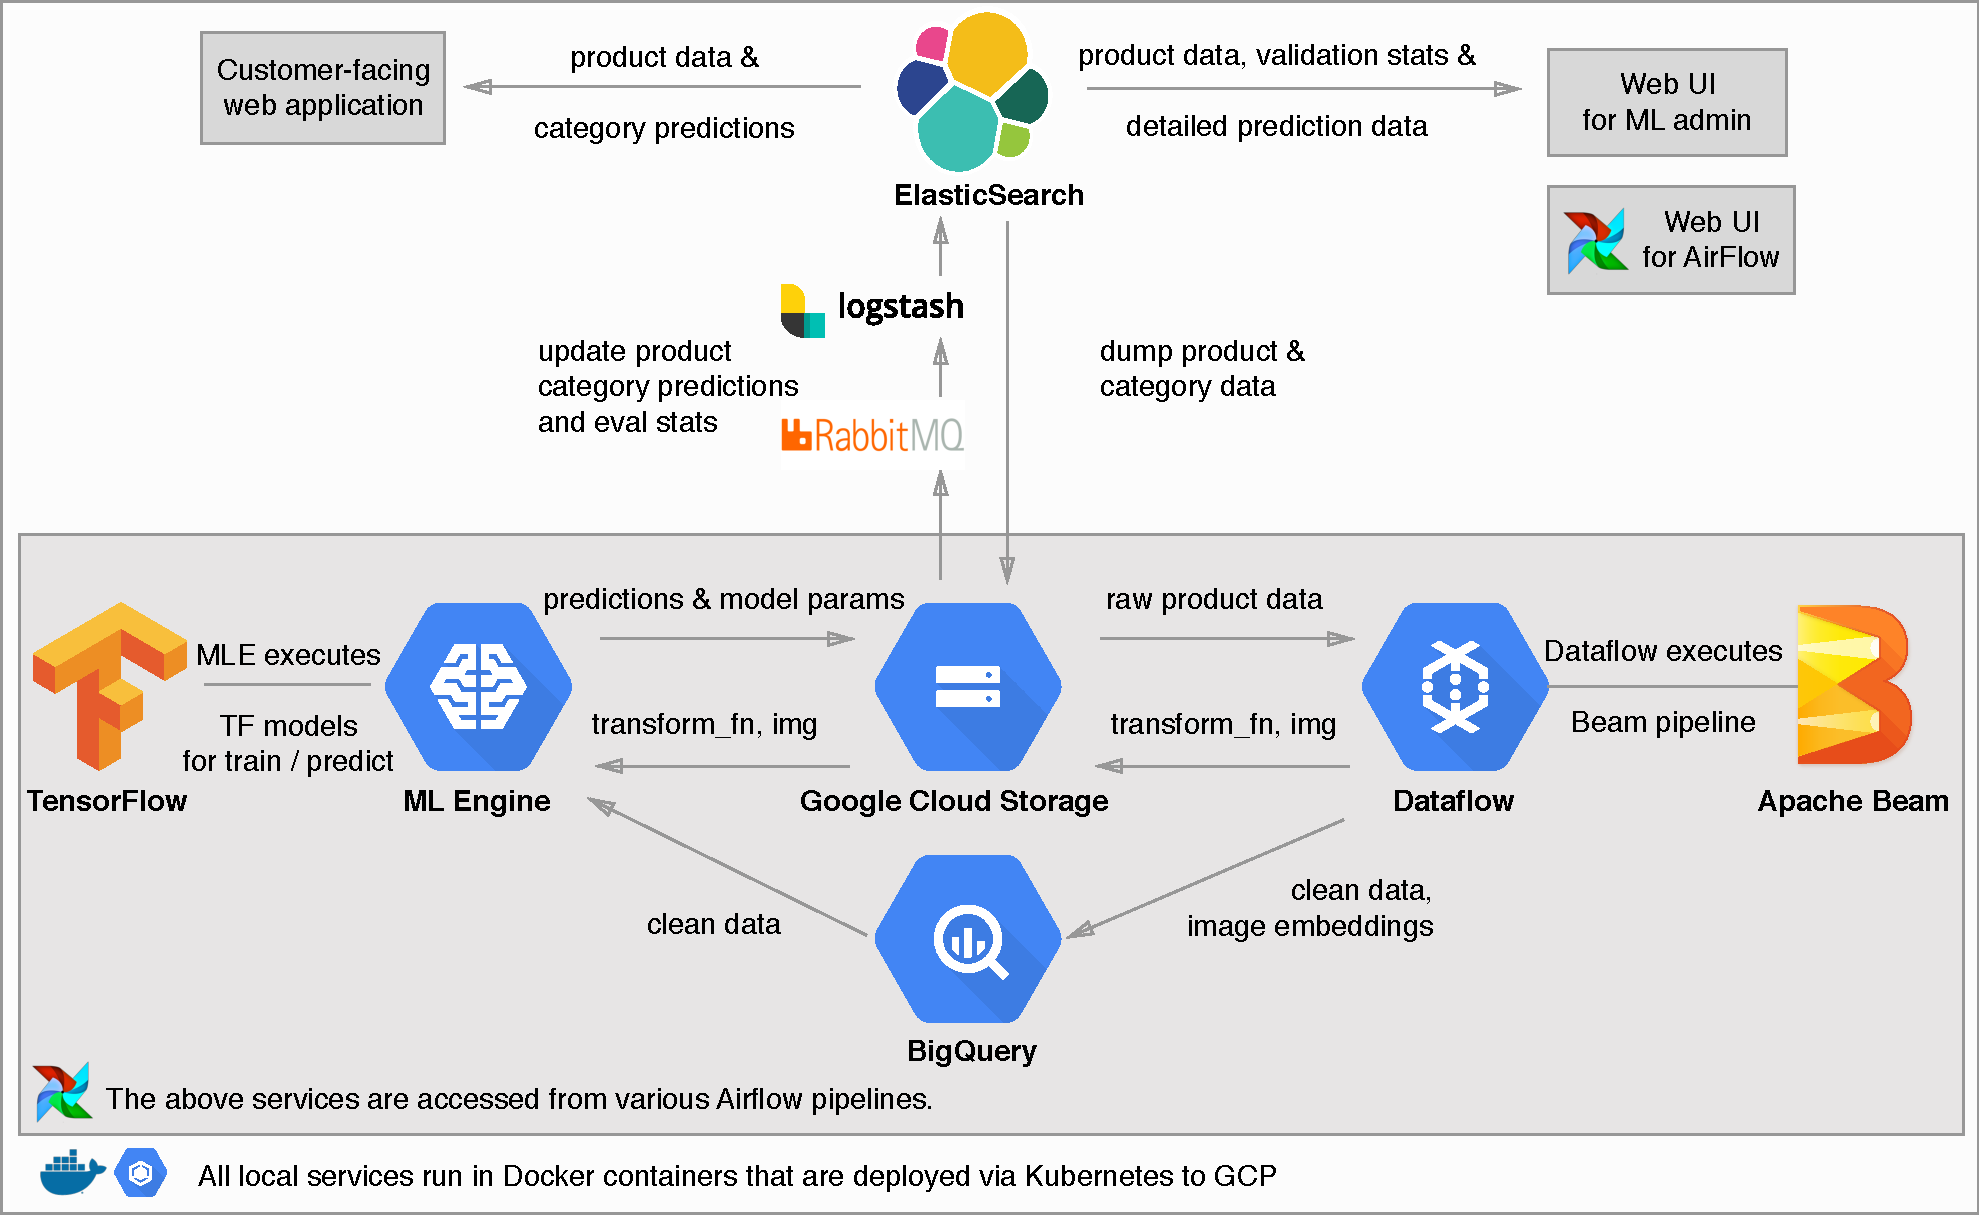
\includegraphics[width=1.4\textwidth]{diagrams/architecture}
  \caption{High-level system architecture of the ML pipeline}
  \label{arch_diagram}
\end{figure}

\subsection{Airflow Pipelines \& Pipeline Runs}

A group of tasks that would need to be run together repeatedly is encapsulated in an Airflow pipeline, which is a directed acyclic graph (DAG) of tasks (also referred to as an AF pipeline).
A DAG is run many times, either based on a schedule or triggered manually.
Figure \ref{fig:af1} shows a screenshot of the most common Airflow pipeline ``cat\_pp\_train\_specific'', which is short for ``categorisation: preprocess and train a specific model''; figure \ref{fig:af2} shows the sub-DAG of the task ``train''.

\begin{figure}
\centering
\begin{minipage}{.48\textwidth}
  \centering
  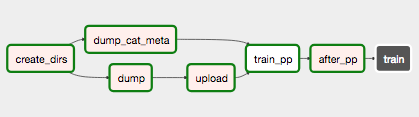
\includegraphics[width=1.0\linewidth]{figures/af_train_specific}
  \captionof{figure}{Airflow DAG: preprocess, train specific model, update statistics. All tasks except for ``train'' have completed, which is not yet scheduled for execution.}
  \label{fig:af1}
\end{minipage}%
\begin{minipage}{.48\textwidth}
  \centering
  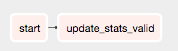
\includegraphics[width=.6\linewidth]{figures/af_train}
  \captionof{figure}{Airflow sub-DAG: train. No task has been scheduled for execution during this run.}
  \label{fig:af2}
\end{minipage}
\end{figure}

Most of our pipelines start by creating directories for our files.
Which files are stored where is configured in a simple file that is accessed by Airflow, Dataflow and TensorFlow (locally or inside MLE); the configuration has placeholders for variables that are determined per run or are specific to a task inside a run.
For example, the location of .tfrecords files is determined by ``\textit{:prefix}/runs/\textit{:run\_id}/ tfrecords/\textit{:objective}\_\textit{:split}.tfrecords'', where \textit{prefix} corresponds to the path to the data directory (either locally or in GCS), \textit{run\_id} is specific to the current run of the pipeline, \textit{objective} is either \textit{rule\_based} or \textit{exclusive}, and \textit{split} is either \textit{train}, \textit{test} or \textit{valid}.
This ensures that all parts of the system look for the same file in the same place, and makes building file paths easier.
All file access in the different parts work equally on a local file system and GCS, which makes it particularly convenient to switch between local experimentation and remote training; in fact, the \textit{prefix} parameter is by default read from an environment variable, which is different in local, Docker and cloud service environments.

A training dataset is identified by its \textit{run\_id}.
The processed .tfrecords, transform function (described below) and metadata is persisted under that run's directory.
Several models can be trained from the same dataset.
The checkpoints of a model are saved under ``\textit{:prefix}/runs/\textit{:run\_id}/checkpoints/\textit{:hparams\_id}/'', where \textit{hparams\_id} identifies a model architecture, as well as what kinds of training objectives and label types it is trained on; during hyperparameter tuning, a unique index is appended to the \textit{hparams\_id} of the model.
As \textit{hparams\_id} encodes only the general model architecture and training objectives, the full set of all hyperparameters is persisted along model checkpoints as a JSON file - for future reference.

\subsection{Dataflow Pipelines}
There are two types of Dataflow pipelines: for preprocessing training data and for calculating product-product visual similarity. Omitting various details, dead-ends and workarounds that were needed due to technical limitations and prior system architecture choices\footnote{which were completely reasonable at the time, when the ML system was not a consideration}, the pipelines had the following tasks:

\subsubsection{Preprocessing}

This pipeline loads the products dumped from ES (as JSON) and preprocesses data according to a configuration file (see section \ref{data_pp}).
Figure \ref{df} shows a screenshot of this pipeline, as visualised by the GCP UI.

In this pipeline, all fields are cleaned of obvious noise and superfluous whitespace.
Text and categorical fields are tokenised and mapped to integer indices, keeping only the top \textit{k} values and also computing TF-IDF scores for text fields.
This is handled by TensorFlow Transform, which persists this token-to-index mapping in a \textbf{transform function} that is saved to GCS at the end of the pipeline.
The transform function is used by a TensorFlow model to convert raw text inputs to a  sparse inputs;
separate pre-processing run will generate a different transform function, with mostly the same tokens mapping to different indices, as the order in which they will be encountered will be different.
The tokenised data is stored to GCS as a sharded .tfrecords files (with one set of files per training objective), a binary file format that TF Transform helps produce; alternatively the raw data could be saved (e.g. as JSON or inside BigQuery) and the transform function inside a TF graph could re-tokenise this raw data at runtime.

\begin{figure}
  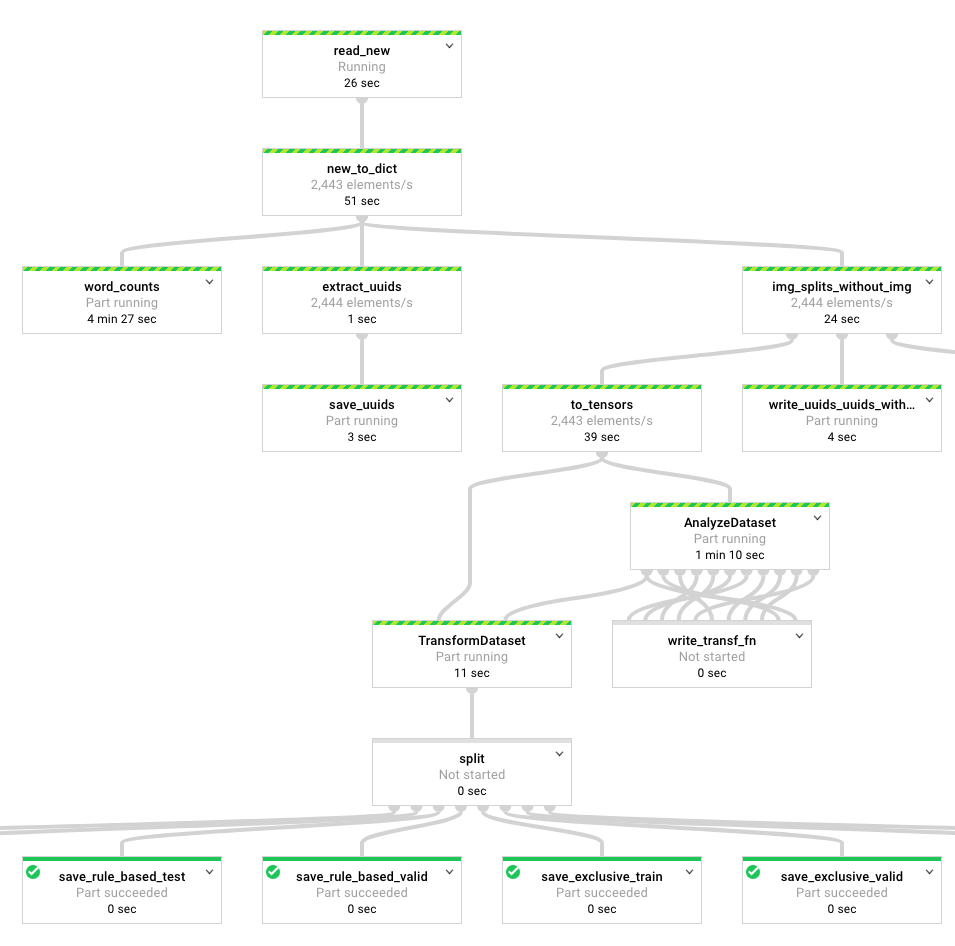
\includegraphics[width=\linewidth]{figures/df}
  \caption{A running Dataflow pipeline of data preprocessing}
  \label{df}
\end{figure}

The pipeline is also responsible for downloading product images, which are saved to GCS as individual files to avoid hitting the content delivery network that stores product images multiple times.
Images are a major bottleneck due to network latency.
To avoid a TF / MLE job from making separate requests to fetch each file individually\footnote{Each request has latency overhead, which compounds quickly when doing million of these.}, Dataflow saves the raw image content into the .tfrecords file; this increases Dataflow execution time, but reduces time and cost overall, as Dataflow is cheaper and easier to parallelise than a MLE job.

A former version of the pipeline also computed image embeddings inside the Dataflow job, but this was inefficient.
We also wanted to have the flexibility to try different models for computing embeddings (e.g. Inception V3, MobileNet, AutoML models) and fine-tuning image models.
Attempts to persist these pre-computed embeddings had severe overheads, and currently the approach is to re-compute these at every time inside MLE, which can leverage a GPU to do it efficiently.

\subsubsection{Visual Similarity}
\label{vis_sim_pp}

The Dataflow pipeline implemented for the experiments described in \ref{exp_sim} relied on image embeddings computed by the preprocessing pipeline.
As explained in section \ref{exp_sim}, it needs to find the \textit{k=100} nearest neighbours of each product based on the cosine similarity of their image embeddings.
The product-product  similarities are the simplest case computed within products that belong to same second level category.
The pipeline read the files output by the preprocessing stage, and partitioned it into datasets by the category predicted in the previous train run (as the new predictions would not be saved in the file).
The per-category image embeddings were merged (using \textit{reduce}) into matrices of image embeddings in a given category, and the top 100 approximate nearest neighbours were extracted for each product using nmslib \cite{nmslib} (as a \textit{map} operation over all the per-category embedding matrices).
The nearest neighbour UUIDs were persisted to GCS and a downstream AF task picked these up and updated ES with these.

This set-up will be replaced in the future.
Computing embeddings in Dataflow is slow, and me way want to enable more flexible ways of restricting the subset of products that are considered (e.g. not just 2nd level category, but a 3rd level category or even globally).
The most flexible approach is one in which nearest neighbours are computed at runtime, i.e. when a product is viewed by a user.
The biggest challenge in such a system is keeping all the image embeddings in memory, which would require 32 GB of memory for the 4 million products we currently have\footnote{$~4000000 * 2048 * 32$ = number of products * embedding dimensionality * 32 bits per number}, and the number of products is likely to increase in the future.

An option worth considering is deploying this as a TensorFlow model to MLE, which reads the embedding matrix in as a sharded tf.Variable; the shards can be distributed on different machines, which is handled automatically by TF.
The input to this model would be just the UUID of the product in question, and the UUID of the category to which the nearest neighbour search is limited; the ``prediction'' of the model would be dot product of the product embedding in question, and all the other product embeddings that are in the given category.
Therefore to get the nearest neighbours of an image embedding, TF would go through all the product embeddings to check for their membership of the given category - but this is fast given all the embeddings are always kept in memory.
The nearest neighbour search will also be precise, which would be prohibitively slow when pre-computing nearest neighbours but should be manageable when done online, as there will be only a handful of requests per second and the dot products are calculated in parallel by multiple workers.
We can also use autoscaling that would increase the number of workers to handle high loads, which would also put all workers to sleep after 15 minutes of inactivity.

\subsection{TensorFlow and ML Engine}

All models were implemented using TensorFlow, using higher level APIs (such as tf.data, tf.estimator and tf.learn) when possible.
This was somewhat challenging, as the high-level APIs were poorly documented, changed even throughout the duration of this project, and it was not clear which APIs are compatible with each other.
Ultimately the only reliable way to understand a class or function was to read its source code.
In many cases these APIs provided almost what was needed, but to support our use case the code was copied from the TensorFlow GitHub repository and adapted to our purpose\footnote{For example, multi-objective learning where each objective potentially changes a subset of the model's variables was not possible due to the way loss from multiple ``heads'' was merged in the current TF APIs. Also some parts had to be rewritten to give us per-class evaluation metrics.}.

The point of entry to the trainer program is the controller.py, which decides based on command line arguments which task to run: train, predict, train and predict, evaluate, export model, etc.
There is a large number of hyperparameters that can be supplied via command-line arguments, with reasonable defaults.

The data was loaded using the tf.data.Dataset API, which provide convenient functions for reading large numbers of files, prefetching, shuffling, batching, and performing arbitrary transformations on the data (such as transforming a set of bytes representing a JPEG image into a 3D tensor of integers).
This works well for simple use cases but is less flexible when for example doing multi-objective learning.
We would like to control roughly how many data points from each objective end up in a batch, or for how long a model is pre-trained on one objective before the second objective is introduced.
Refer to section \ref{multiobj} for a description of two approaches that were tried.
In general, the trainer program would use tf.data.Dataset class to build an \textit{input function} for either training or evaluating, and the input function would be supply data points for the train loop.

TensorFlow models were built using the tf.estimator.Estimator class by providing a custom \textit{model function}.
The model function would dynamically build the model based on the \textit{model type} (deep / linear), \textit{input type} (these are listed in section \ref{exp_models}), \textit{training objectives} and \textit{hyperparameters}.
An input type determines which input features are used and how they are represented, while a training objective determined which training dataset, loss function and evaluation metrics were used.
Both input types and training objectives had simple configuration files dictating their behaviour, which made adding new training objectives and experimenting with different model architectures easy.

Training was handled by the tf.estimator.train\_and\_evaluate function.
It loads a model from the checkpoint directory if present, and trains the model for a specified number of steps (or until the input function terminates).
It also periodically saves model checkpoints to GCS, and handles writing TF summary operations that are needed for data visualisations using TensorBoard\footnote{TensorBoard is a web interface for visualising the variables and metrics a TensorFlow train run produces; many of the visualisations in the following sections are taken from Tensorboard.}

\section{Experiments, Evaluation \& Results}
\label{exp}

There are many kinds of experiments conducted; the experiments, their evaluation and results are explained under the same subsection.
In section \ref{exp_sim} three visual similarity approaches are described and subjectively evaluated;
in section \ref{exp_models} we describe all the models that were trained to reproduce the behaviour of the rule-based system;
how multi-objective learning was used to improve the accuracy of individual training objectives is described in section \ref{multiobj};
finally, our efforts to reduce label complexity using active learning is described in section \ref{exp_al}.

\subsection{Visual Similarity}
\label{exp_sim}

Three approaches were tried for computing visual similarity.
In the first case, an approximate nearest neighbour method \cite{nmslib} was used on the image embeddings (as described in section \ref{vis_sim_pp}) and the top 100 predictions were saved to ElasticSearch.
In the second approach, the embedding vectors were discretised according to \cite{vec_fulltext} (as described in section \ref{bg_sim}) and inserted to ElasticSearch as strings of space-delimited tokens; standard ElasticSearch fulltext search was used on these token strings to get the nearest neighbour for a given product.
The third approach combined the similarity scores of the second approach and the original ElasticSearch title matching, as a single ElasticSearch query.

\subsubsection{Evaluation \& Results}

The evaluation of similarity scores is difficult, since it is inherently somewhat subjective.
A common approach is to hand-label triplets of images Q, A, B with four choices: (1) both A and B are similar to query image Q, (2) both A and B are dissimilar to Q, (3) A is more similar to Q than B, and (4) B is more similar to Q than A.
These labeled triplets can be ranked using with similarity precision (percentage of triplets correctly ranked) and score at top K (see \cite{imgsimfineg}).
Creating this dataset of triplets would be a very time-consuming process. Therefore evaluation was done entirely subjectively.

Comparing the similarity between the former ElasticSearch title (ES title) matching and the new approximate nearest neighbour (ANN) search was straightforward - one look at the results was enough to confirm that the embedding-based approach outperforms title matching.
Figures \ref{shirt_es} and \ref{shirt_nmslib} show the nearest neighbours according to ES title and ANN, respectively; the image embeddings nicely pick up the pattern on the shirt, as well as the general style, but also seems to prefer pictures with no fashion model.
For some clothing categories this worked remarkably well, but with categories that had more varied products within it, there were occasional odd results.
For example, in the ``Hiking'' category, the nearest neighbours of sleeping bags could be items with seemingly similar shapes, such as a flashlight that a very zoomed-in product photo that had similar contours as an unrolled sleeping bag.
Another example of this is given in figure \ref{chair_nmslib}, which mostly returns chairs that are indeed visually and even functionally very similar to the chair in question - more so than the ElasticSearch title match seen in \ref{chair_es} - but also returns tables with similar legs; this is understandable, given that nearly half of the surface area of these images is covered by these foldable legs, which are visually quite unique.
This problem can mostly be mitigated by having more fine-grained product categories and restricting the nearest neighbour search to those more specific categories.
The nearest neighbour similarity search may pick up qualities of the image that are not related to the product in question, such as background or fashion model; this is un-intended but is acceptable, and it could be argued creates a product listing which is more homogenous and therefore more aesthetically pleasing.

The second approach of discretised and tokenised image embeddings had mixed results.
The returned nearest neighbours were reasonable, but subjectively felt inferior to the ones computed from the raw image embeddings using ANN.
At times it felt like some aspect of the appearance dominated, which is understandable considering a lot of precision is lost when discretising the embeddings, and there is no theoretical justification why a TF-IDF score of these arbitrarily discretised tokens should behave similarly as a dot product between the original vectors.
With enough precision (using several discrete intervals per embedding dimension) this may well work, but this would incur a considerable performance overhead (when indexing and querying).
A hybrid approach was also attempted, where the tokenised version is used to come up with a small set of candidate nearest neighbours, which are used for a precise nearest neighbour calculation; the latter was implemented as an ElasticSearch plugin that performed dot products on the raw embedding vectors, but this was not a scaleable solution and did not subjectively lead to particularly good similarity results.

The third approach of combining the existing title matching and discretised and tokenised vectors was somewhat successful.
As seen in figure \ref{chair_tokenised}, the title matching ensures that top results are at least about the same kind of items (chairs) while the tokenised embedding query returns products that share some visual similarity (mostly the legs of the chair).
This approach still suffered from similar problems as the second approach - poor performance and somewhat inconsistent visual similarity - while introducing an additional complication of finding a good weighting between the title and visual scores.
Given that there was no efficient way to evaluate the different weightings, it was decided to use raw image embeddings for visual similarity (either as an ANN or a precise realtime version).

\begin{figure}
  \centering
  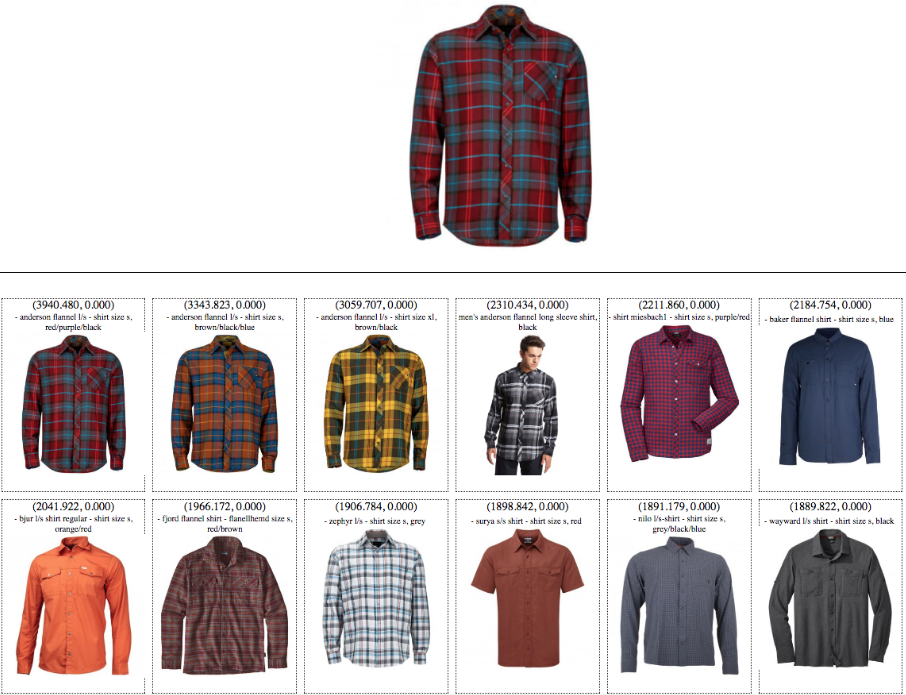
\includegraphics[width=0.8\linewidth]{figures/compare/shirt_es}
  \caption{Nearest neighbours based on ElasticSearch title matching (TF-IDF-like)}
  \label{shirt_es}
\end{figure}
\begin{figure}
  \centering
  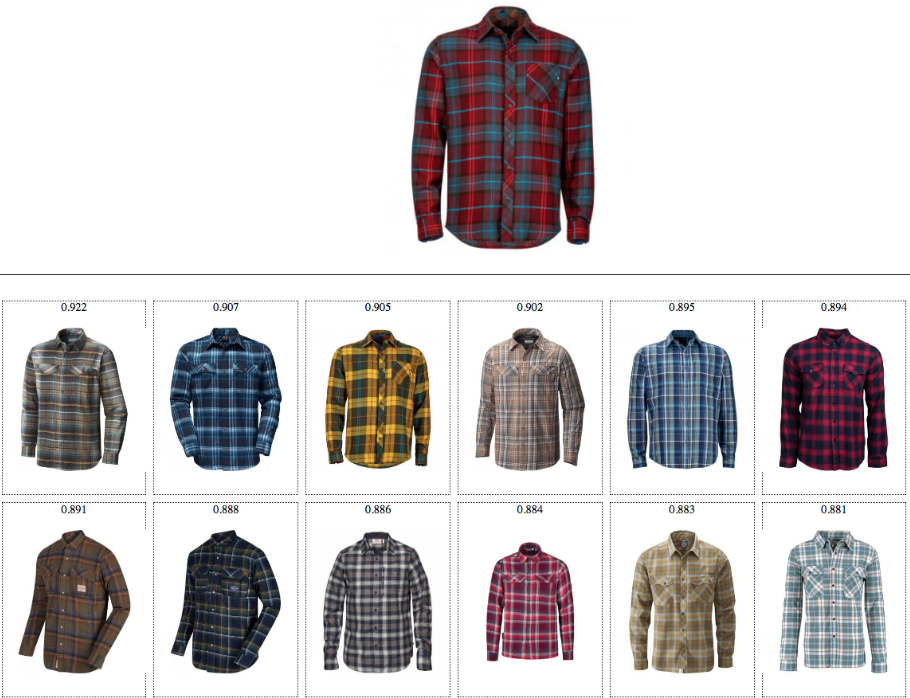
\includegraphics[width=0.8\linewidth]{figures/compare/shirt_nmslib}
  \caption{Nearest neighbours based on ANN search of image embeddings}
  \label{shirt_nmslib}
\end{figure}

\begin{figure}
  \centering
  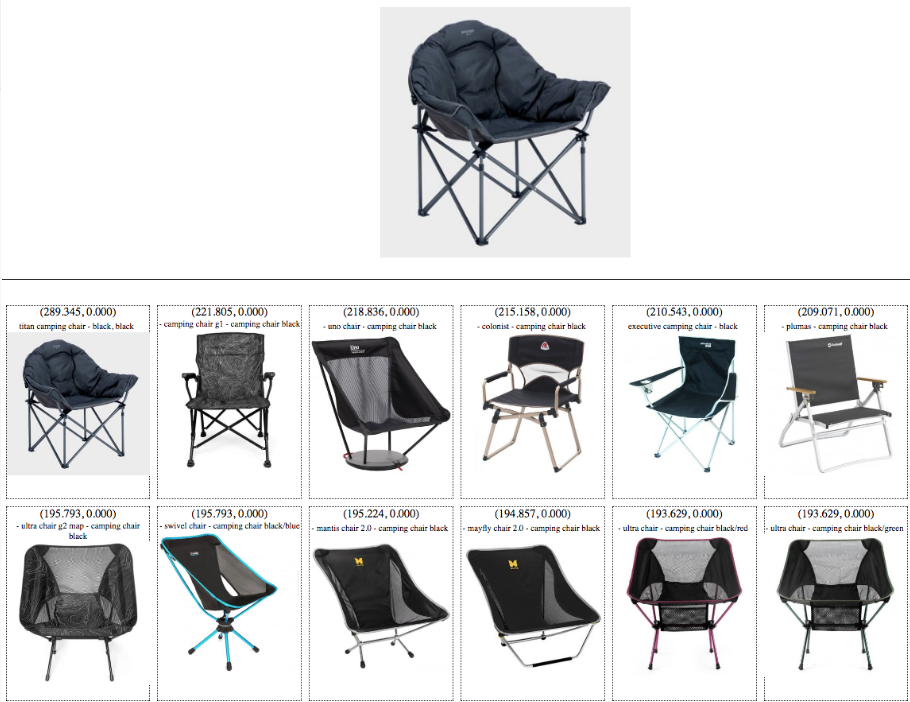
\includegraphics[width=0.8\linewidth]{figures/compare/chair_es}
  \caption{Nearest neighbours based on ElasticSearch title matching (TF-IDF-like)}
  \label{chair_es}
\end{figure}
\begin{figure}
  \centering
  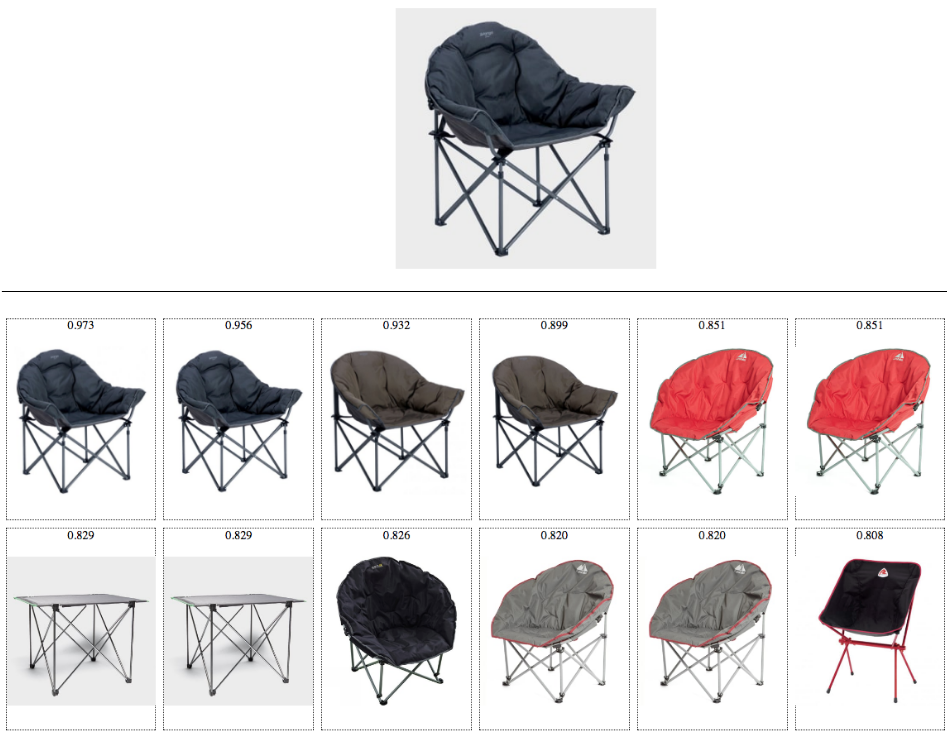
\includegraphics[width=0.8\linewidth]{figures/compare/chair_nmslib}
  \caption{Nearest neighbours based on ANN search of image embeddings}
  \label{chair_nmslib}
\end{figure}
\begin{figure}
  \centering
  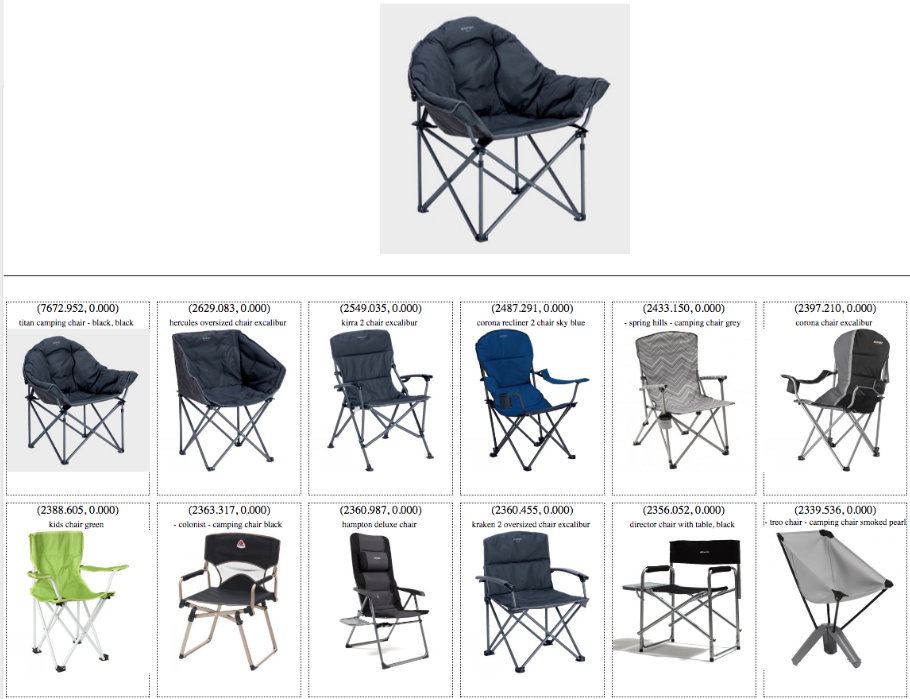
\includegraphics[width=0.8\linewidth]{figures/compare/chair_tokenised}
  \caption{Nearest neighbours based on fulltext search on discretised/tokenised image embeddings as in \cite{vec_fulltext}. Here scores from the title and image embedding fields was combined.}
  \label{chair_tokenised}
\end{figure}

\subsection{Independent Models}
\label{exp_models}

Several models were trained on the rule-based labels to find out which models can best replicate its behaviour.
In section \ref{widedeep} we describe the first model that was trained as a baseline.
The different input features and how these were represented is described in section \ref{model_comb}, along with how linear and deep modelds were trained from these input representations.
Section \ref{tuning} describes how hyperparameters were selected, and two attempts at tuning these programmatically.


\subsubsection{Evaluation}

Many metrics can be used to evaluate \textbf{multi-label classification}:

\begin{itemize}
  \item TP, TN, FP, FN: true positives, true negatives, false positives, false negatives,
  \item accuracy: $\frac{TP + TN}{FP + FN}$, fraction of correct predictions,
  \item precision: $\frac{TP}{TP + FP}$, fraction of positive predictions that were correct,
  \item recall: $\frac{TP}{TP + FN}$, fraction of positive labels that were correctly ``recalled'',
  \item F1: $2\frac{precision * recall}{precision + recall}$, harmonic average of precision and recall,
  \item TPR = precision: $\frac{TP}{TP+FP}$, true positive rate,
  \item FPR: $\frac{FP}{FP+FN}$, false positive rate,
  \item ROC AUC: the area under the curve of TPR plotted against FPR.
  \item PR AUC: the area under the curve of precision plotted against recall.
\end{itemize}

In our case, an overwhelming number of labels are negative, therefore a very simple predictor (that predict ``negative'' for every product / category) would have an accuracy near 99\%; ROC AUC is not suitable for the same reason, as there would be no false positives.
Precision and recall are useful measures to understand the model: it is expected to see a sharp increase of precision and decrease of recall as the model learns to predict ``negative'' for most classes, followed by a gradual increase of recall as the model learns to predict ``positive'' for the correct classes.
Precision and recall are competing metrics: increased precision tends to lead to decreased recall and vice versa, therefore models which combine the two are suitable for evaluating multi-label prediction problems with unbalanced classes.
While F1 score gives the harmonic mean of precision and recall at a given threshold, PR AUC paints a more complete picture by showing what the ratio would be at all the threshold values\footnote{There are infinitely many threshold values in the range 0 ... 1, so naturally we consider a small number of threshold values when approximating AUC.}.
Therefore, all evaluation of multi-label classification is based on PR AUC, i.e. when choosing between model architectures or hyperparameters, a model with a higher PR AUC is preferred.

For \textbf{multi-class classification}, accuracy is still a reasonable measure.
Even though classes are imbalanced (``Dresses'' has more products than ``Travel Books''), there is no single dominant class that could be used as a shortcut by the model.
On the other hand, similar problems arise with evaluating multi-class problems where there is potentially overlap between some classes: the metric would give a low score even if the model predicted a semantically very similar class, or a more general class instead of the more specific one it was labelled as.
Therefore a manual evaluation of the misclassified products is needed to determine whether the error rate is caused by the ambiguity of the classes or by problems with learning.

\subsubsection{Baseline Model: Wide \& Deep}
\label{widedeep}

As described in section \ref{bg_wide_deep} ``Wide \& Deep'' consists of two models that are trained jointly using stochastic gradient descent: a deep and a shallow neural network which both predict the same set of binary outputs.
The original idea of Wide \& Deep was to use the wide component for feature crosses (e.g. of two categorical values), but in our experiments the wide component received mostly just the 1-hot encoded categorical inputs while the wide component received the same inputs as random embeddings (or as pre-computed image embeddings extracted with Inception V3 that is pre-trained on ImageNet).

Initial experiments with this model were done on a dataset of roughly 800 000 products which were labeled by the rule-based system\footnote{The database in the client company was in constant flux, so the training set sizes depended on how many labels the rule based-system had assigned to the current database}.
The data was partitioned into a train (\textasciitilde80\%), validation (\textasciitilde10\%) and test (\textasciitilde10\%) sets in the Dataflow preprocessing pipeline based on a pseudorandom number generator - assign the product in question to the dataset if the random number is in the range 0 ... 0.8, 0.8 ... 0.9, 0.9 ... 1.
This allowed us to use parallel data preprocessing where workers do not need to be aware of the index of the data point it is processing or what the other workers are doing; due to the randomness the dataset split boundaries will not be exact (e.g. test and validation sets may end up with 12\% and 8\% of products), but this is acceptable given the relatively large dataset size.
The train set was used to train the model, and the validation set was used to evaluate the model periodically as it was trained - during individual training runs and during hyperparameter tuning.
The test set was held out for evaluating the model after hyperparameter tuning, but was not used in this case.

\paragraph{Results}
The PR AUC on the 800,000-item dataset for this model after hyperparameter tuning was 0.9981 (see section \ref{tuning} for a full description of the set-up).
A manual examination of the predictions revealed that the top predictions for most categories was high-quality, but there was a large number of products below the decision boundary that actually belonged above it.
A later run of the model on 1 600 000 products gave an PR AUC of 0.8647; this was using the hyperparameters that the tuning step produced, so it is likely that the decreased AUC PR score is caused by a bug\footnote{Three possible explanations come to mind: (1) the initial PR AUC was artificially high as some of the test set products ended up in the training set; (2) when migrating from the 800k dataset to the 1.6M dataset, the image embeddings were transferred over as an attempted optimisation approach; (3) the model was overfitting, 10 epochs of 1.6M is effectively 20 epochs of 800k products (the fact that there were more products does not necessarily matter, because labels were assigned simplistically from keyword matches on the title).}.
There were occasional odd results from the model once it was trained on the 1.6M dataset; it was hard to tell which part of the model was causing it, or even whether all the input features are actually improving predictive power; therefore, a more systematic approach was tried, explained in the next section.

\subsubsection{Input Representation \& Model Type Combinations}
\label{model_comb}

To assess which features are most useful for learning the rule-based objective, different features were grouped into \textit{input types}, shown in table \ref{input_types}.
The columns represent the input feature; refer to \ref{data_pp} for the full feature names and their description.
The entries in the table show how each input feature was represented: \textit{emb} for for categorical features that are represented as random embedding vectors (which are updated during SGD), \text{emb avg} for multi-token fields where tokens are represented as random embeddings and the input feature is a weighted sum of these embeddings\footnote{Each embedding vector is weighted by the number of times it appears in the input feature, and divided by the L2 norm of the token counts; this gives good results for bag-of-words inputs according to TensorFlow documentation:
\newline
https://www.tensorflow.org/api\_docs/python/tf/feature\_column/embedding\_column}.
Feature columns marked with \textit{u.s.enc} have been converted from raw text into dense embedding vectors of size 512 using a pre-trained model Universal Sentence Encoder \cite{uni_sent_enc}; cells marked with \textit{mobilenet} and \textit{inceptionv3} have respectively extracted image embeddings of size 1280 and 2048 using the Mobilenet \cite{mobilenet} and InceptionV3 \cite{inceptionv3} models that were pre-trained on the ImageNet challenge; these embedding models were used via TensorFlow Hub\footnote{TensorFlow Hub is a collection of TensorFlow models that are pre-trained on some other task and can be used as a feature extractor or as an initialisation for a model that is fine-tuned: https://www.tensorflow.org/hub/}.
Pre-trained models were used only as feature extractors, i.e. were not fine-tuned on our data.

\begin{figure}
  \centering
  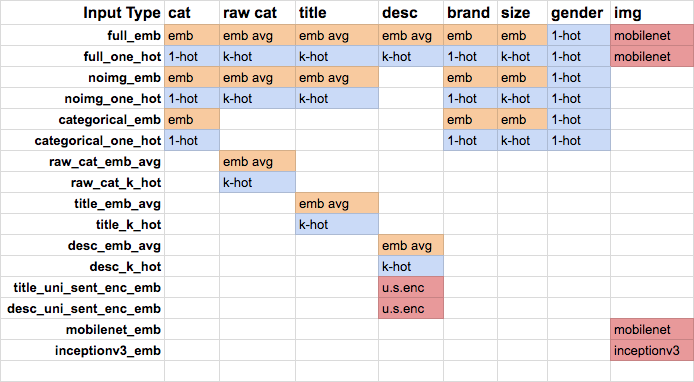
\includegraphics[width=\linewidth]{figures/input_types}
  \caption{Input types. Orange: embedding representation, blue: 1-hot or k-hot, red: embedding extracted with a pretrained deep network.}
  \label{input_types}
\end{figure}

Two model types were used to train with each of these 16 input types: linear and deep.
Like in the case of the baseline model, the \textasciitilde1.6 million data points were split into train/validation/test sets (80\%/10\%/10\%); train and validation sets were used during individual training runs and hyperparameter tuning.
All 32 combinations of input and model type were trained using hyperparameters listed in section \ref{tuning}; these were selected based on what worked well on the baseline model and in general ``seemed reasonable''.
The initial plan was to use automatic hyperparameter tuning on a few model/input types, but the tuning failed to produce good results.
The PR AUC on the validation set is shown in figure \ref{pr_auc_all}, where each model is trained for 300 000 batches, which is roughly 6 epochs.

\begin{figure}
  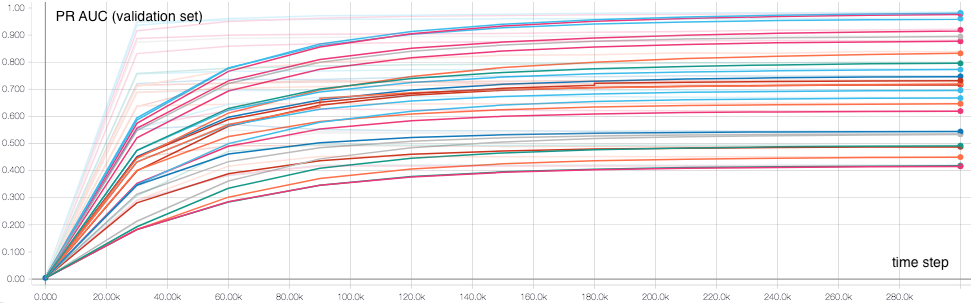
\includegraphics[width=\linewidth]{figures/pr_auc_all}
  \caption{PR AUC of all combinations of input and model types; x axis = train step (batch number), y axis = PR AUC. Refer to figure ... for exact scores.}
  \label{pr_auc_all}
\end{figure}


\subsubsection{Hyperparameter Selection \& Tuning}
\label{tuning}

\subsection{Multi-Objective Training}
\label{multiobj}

pre-train vs train exclusive from the start
both vs interleave
from rb to ex

\subsection{Active Learning}
\label{exp_al}

% \subsection{Performance Optimisation}
% \label{performance}
